\documentclass{article}
\usepackage{graphicx}
\usepackage[nomarkers]{endfloat}
\renewcommand{\efloatseparator}{\newpage}
\renewcommand{\listoffigures}{} % but suppress these lists
\renewcommand{\listoftables}{} % suppress these lists
\begin{document}

\begin{figure}[h!]
  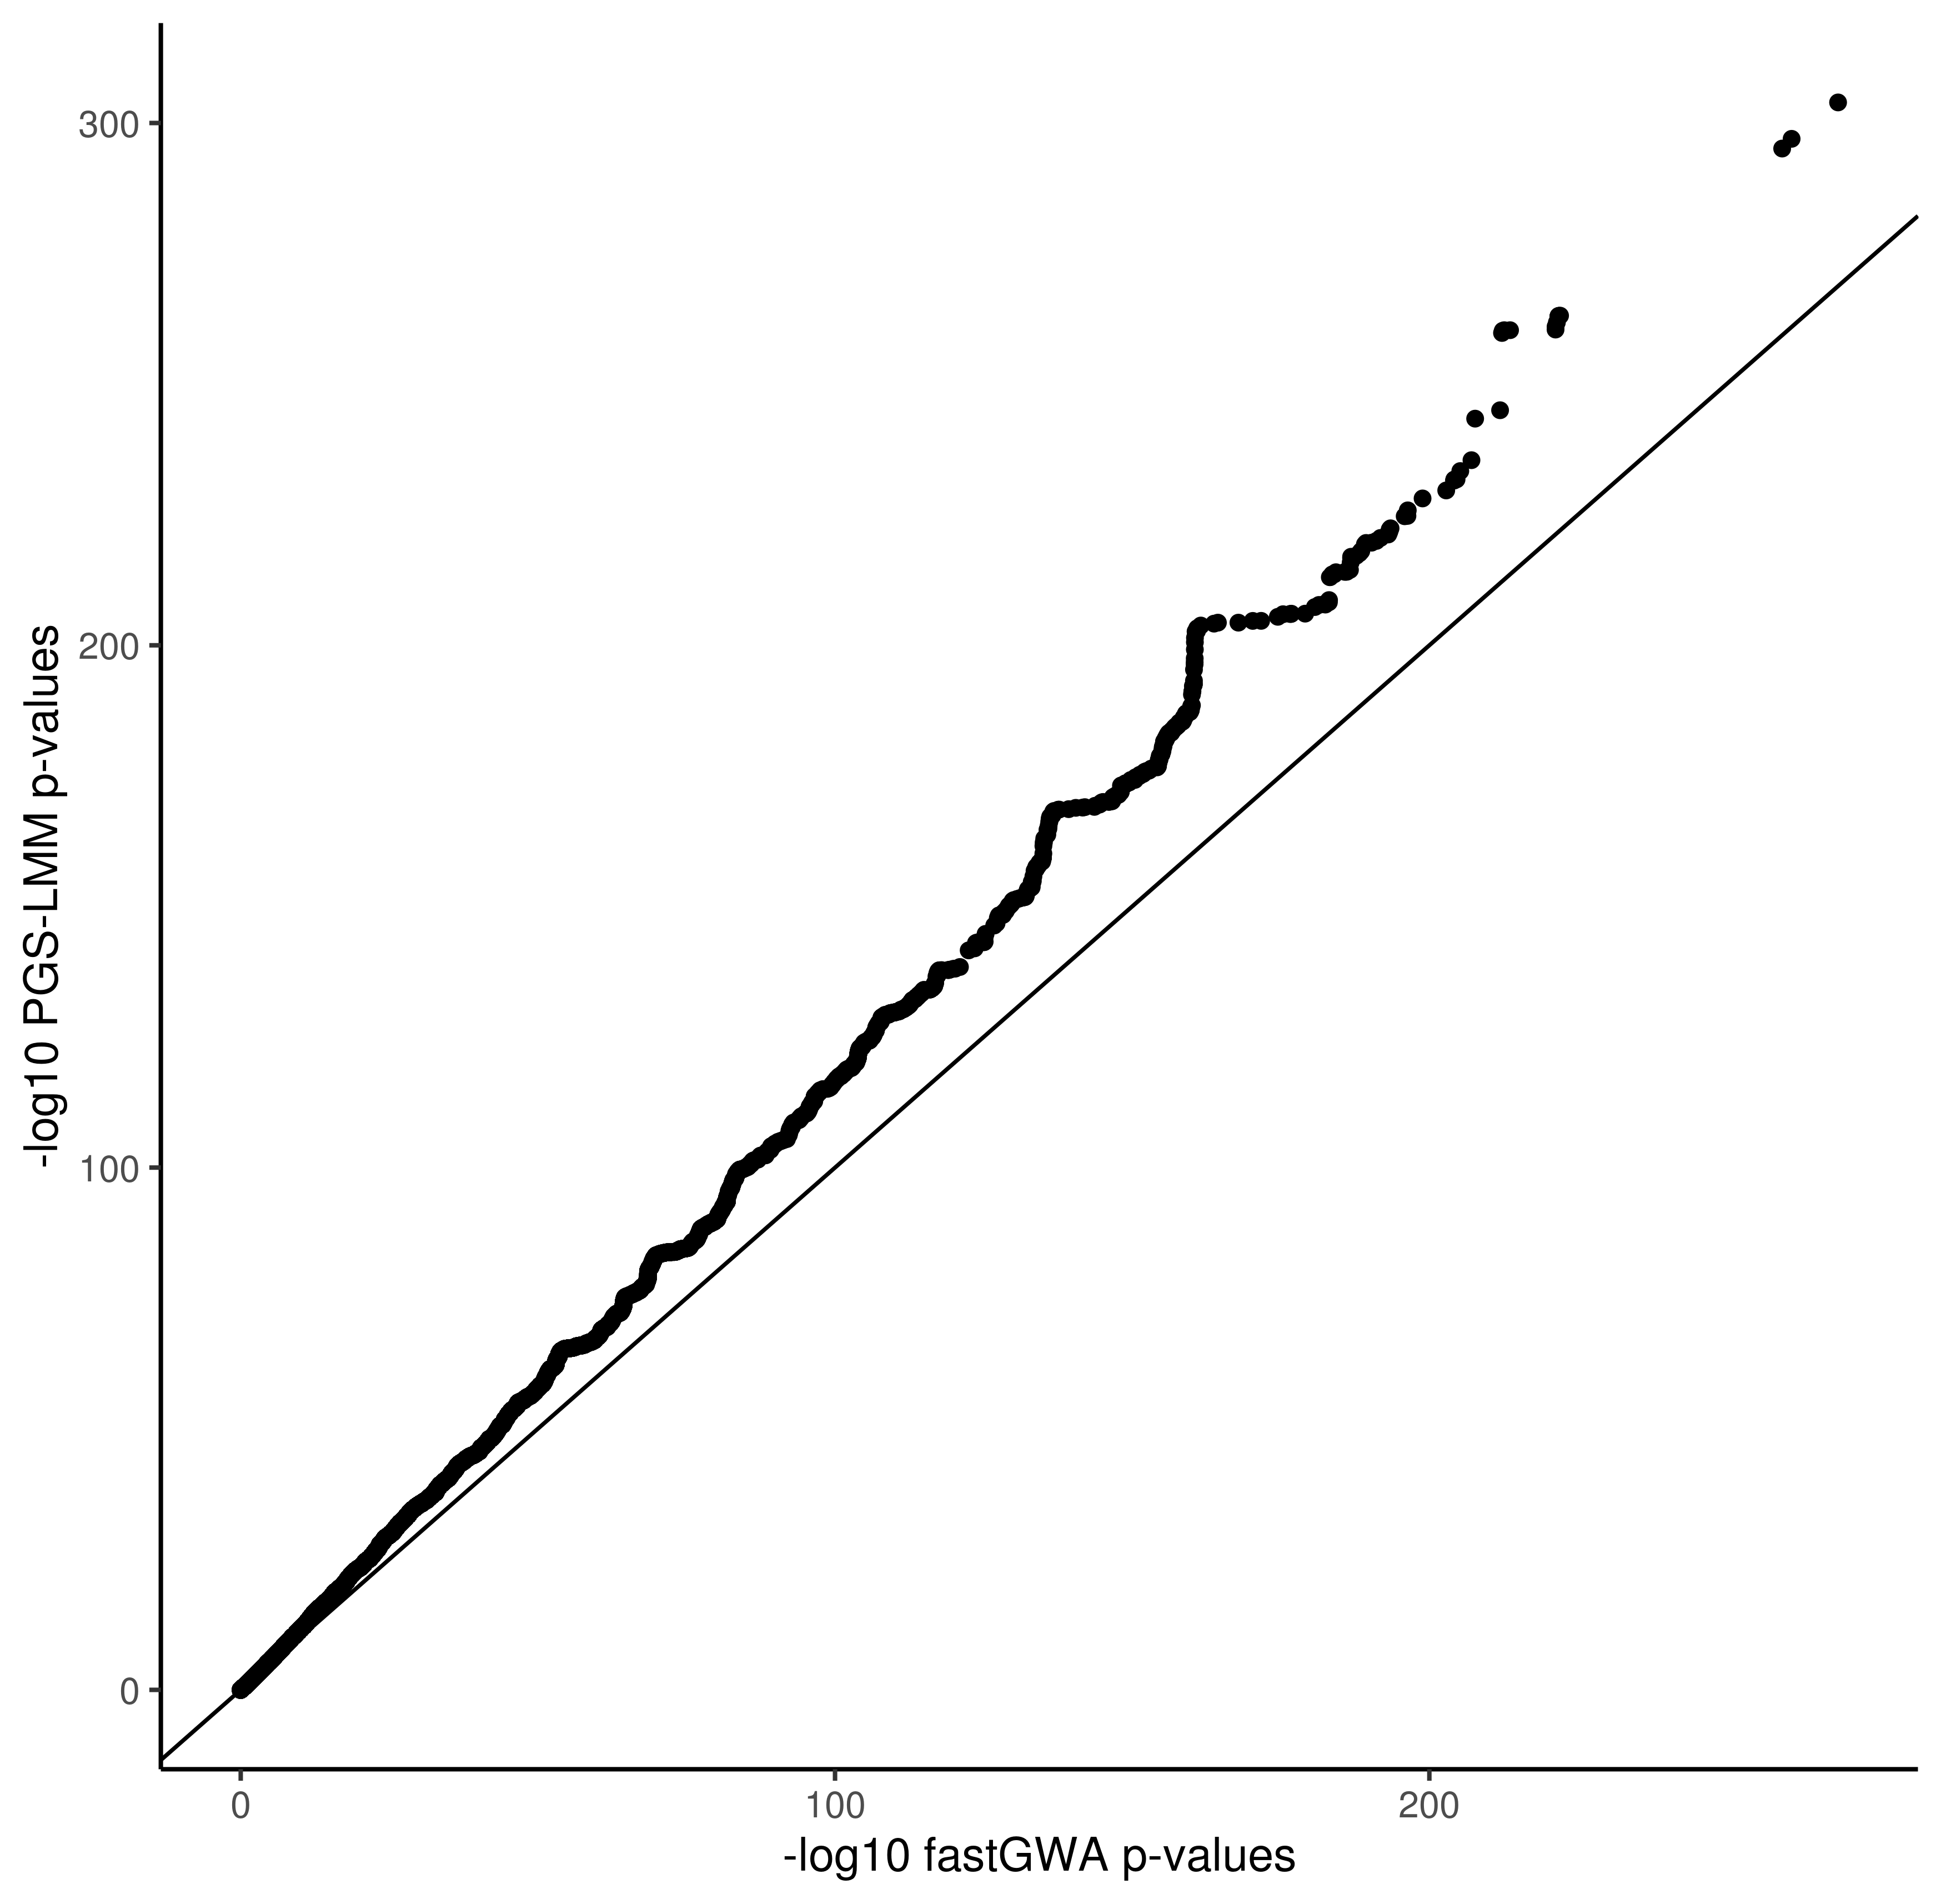
\includegraphics[width=0.85\textwidth]{images/SFig1.png}
  \caption{Distribution of variant significance for PGS-LMM (y-axis) and fastGWA (x-axis)}
\end{figure}

\begin{figure}[h!]
  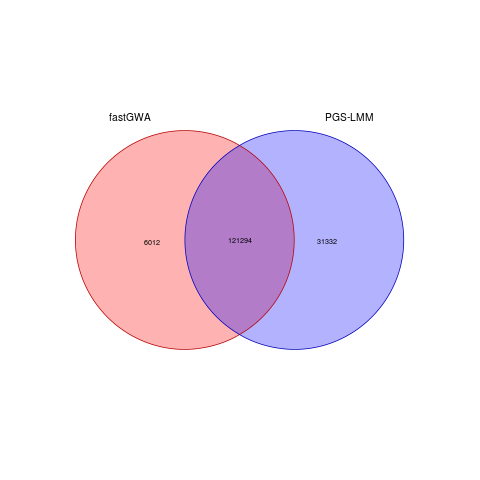
\includegraphics[width=0.85\textwidth]{images/SFig2.png}
  \caption{Venn diagram of significant variants identified by both FastGWA and PGS-LMM}
\end{figure}

\begin{figure}[h!]
  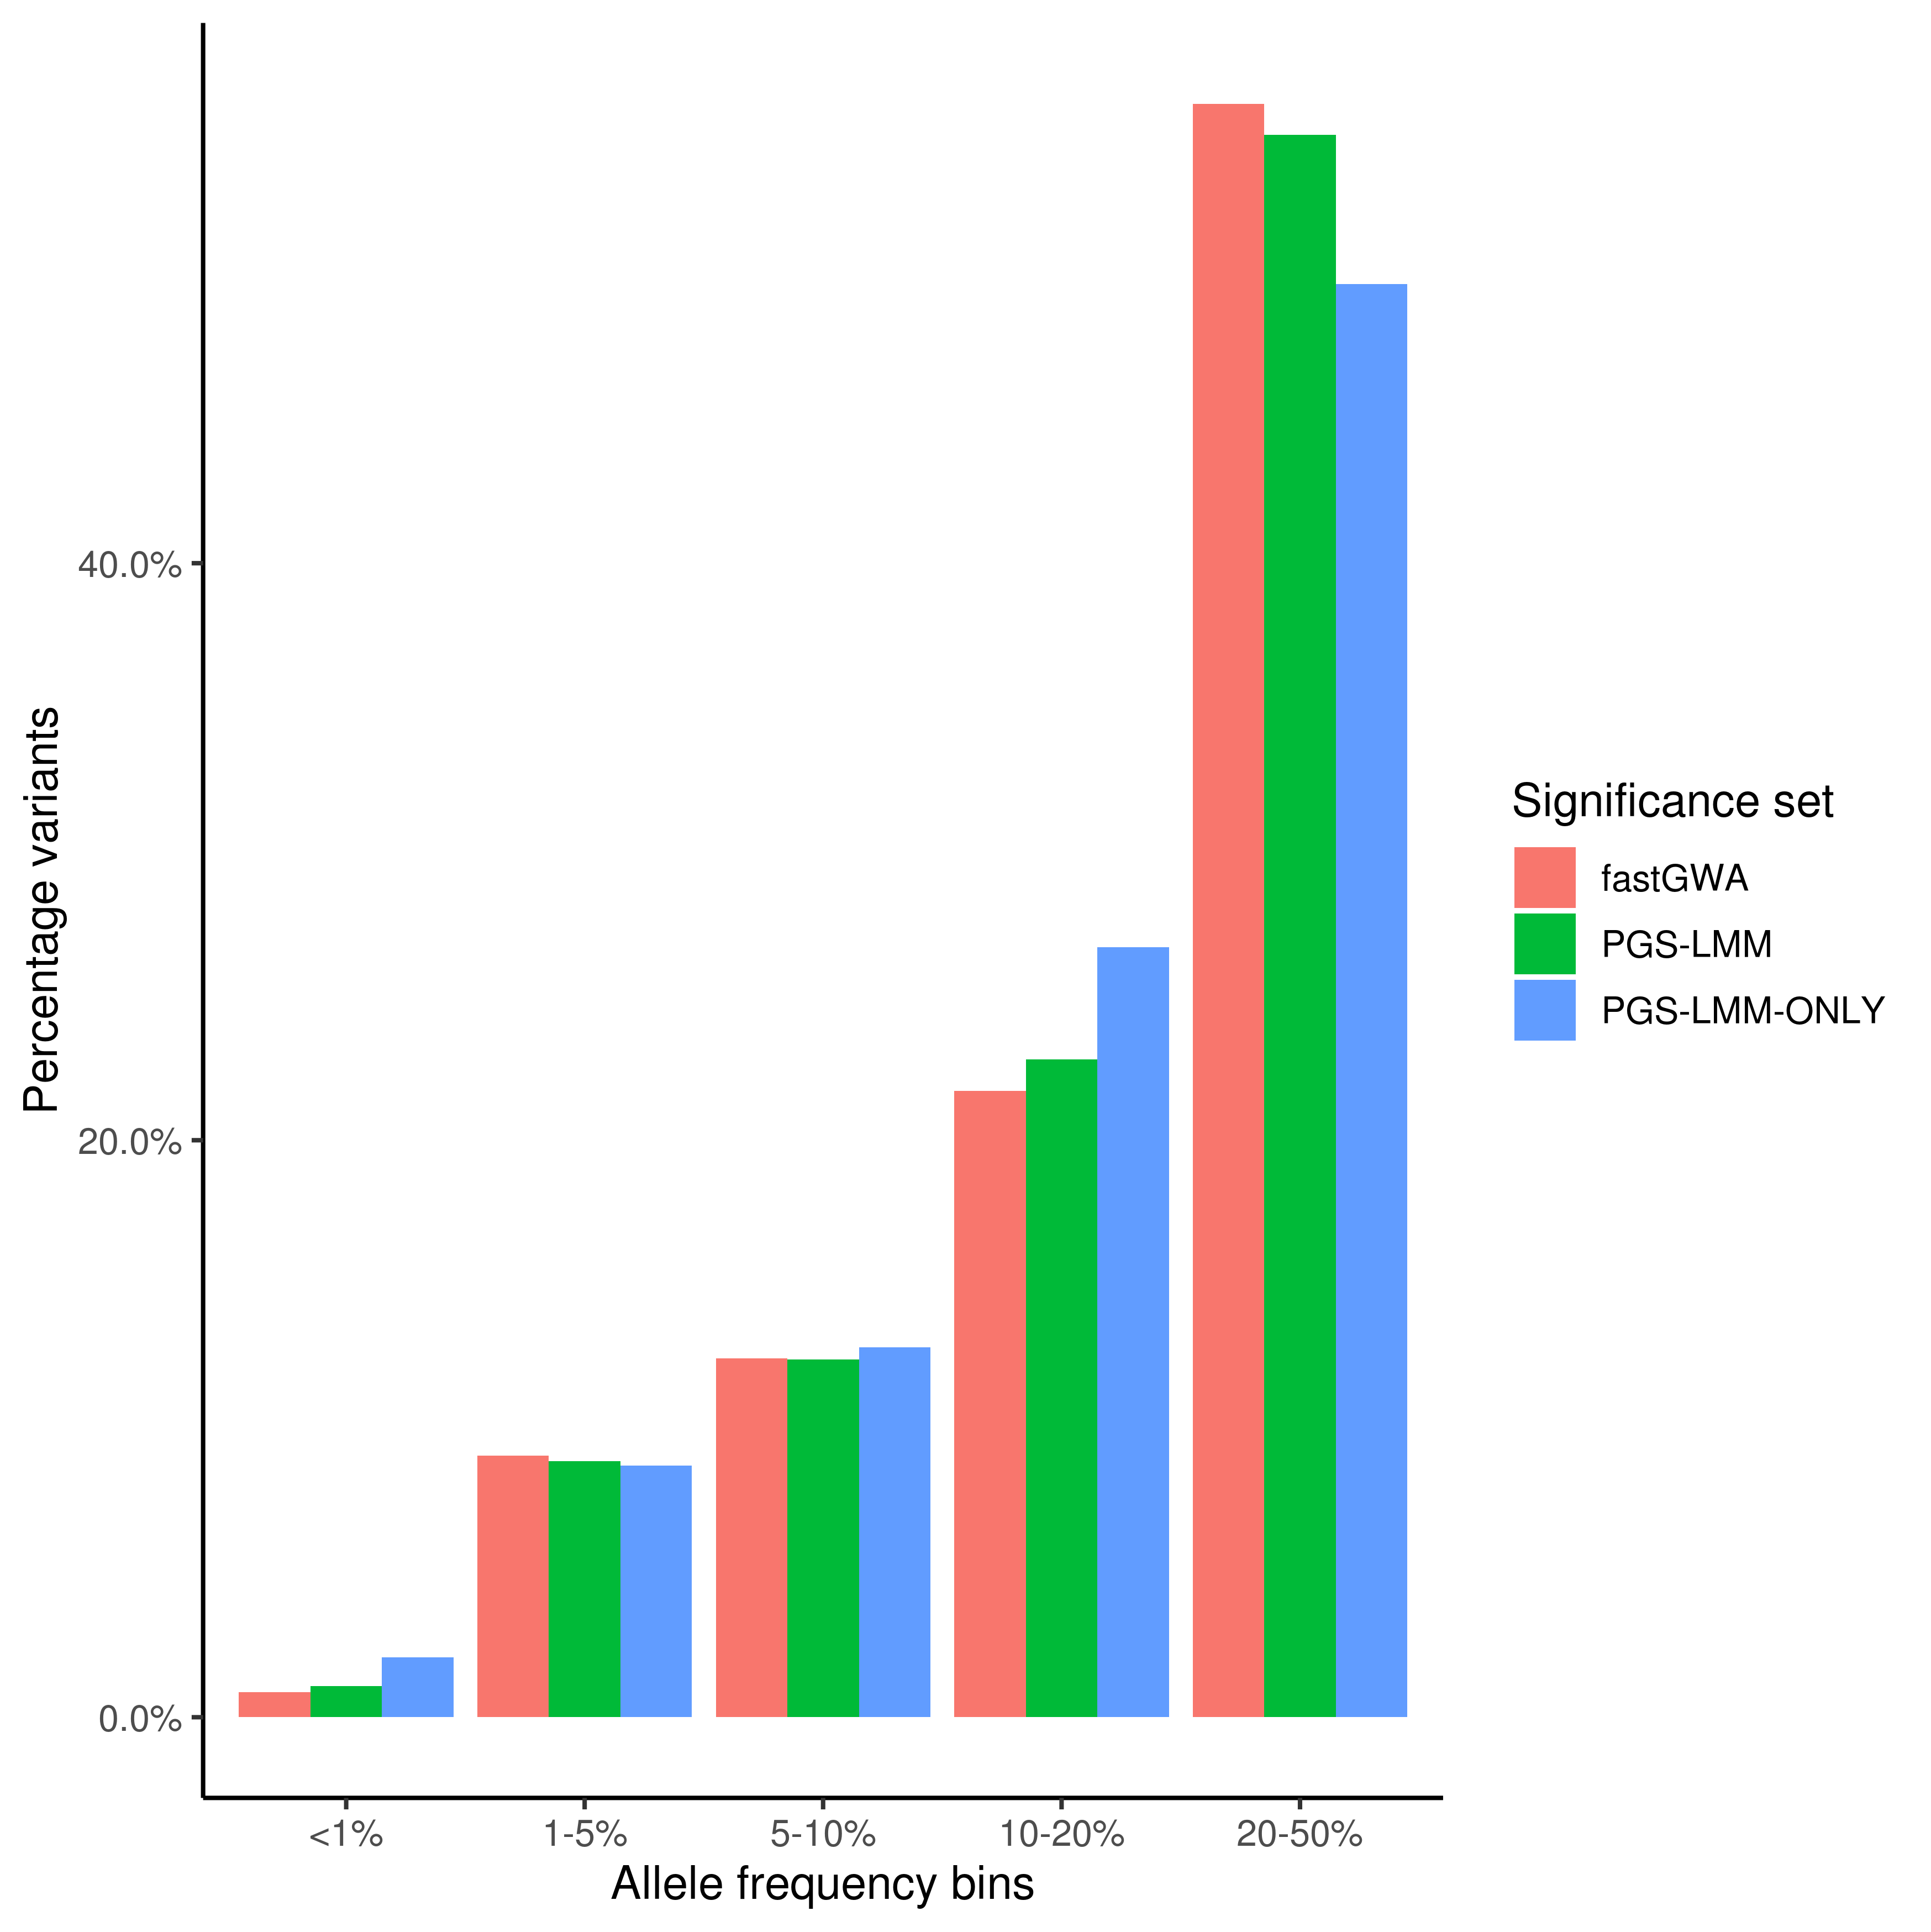
\includegraphics[width=0.85\textwidth]{images/SFig3.png}
  \caption[MAF plot]{Minor allele frequency of significant variants identified by the fastGWA method (red), MAF of variants identified by PGS-LMM (green) and variants identified by the PGS-LMM method and not fastGWA (blue)}
\end{figure}

\begin{figure}[h!]
  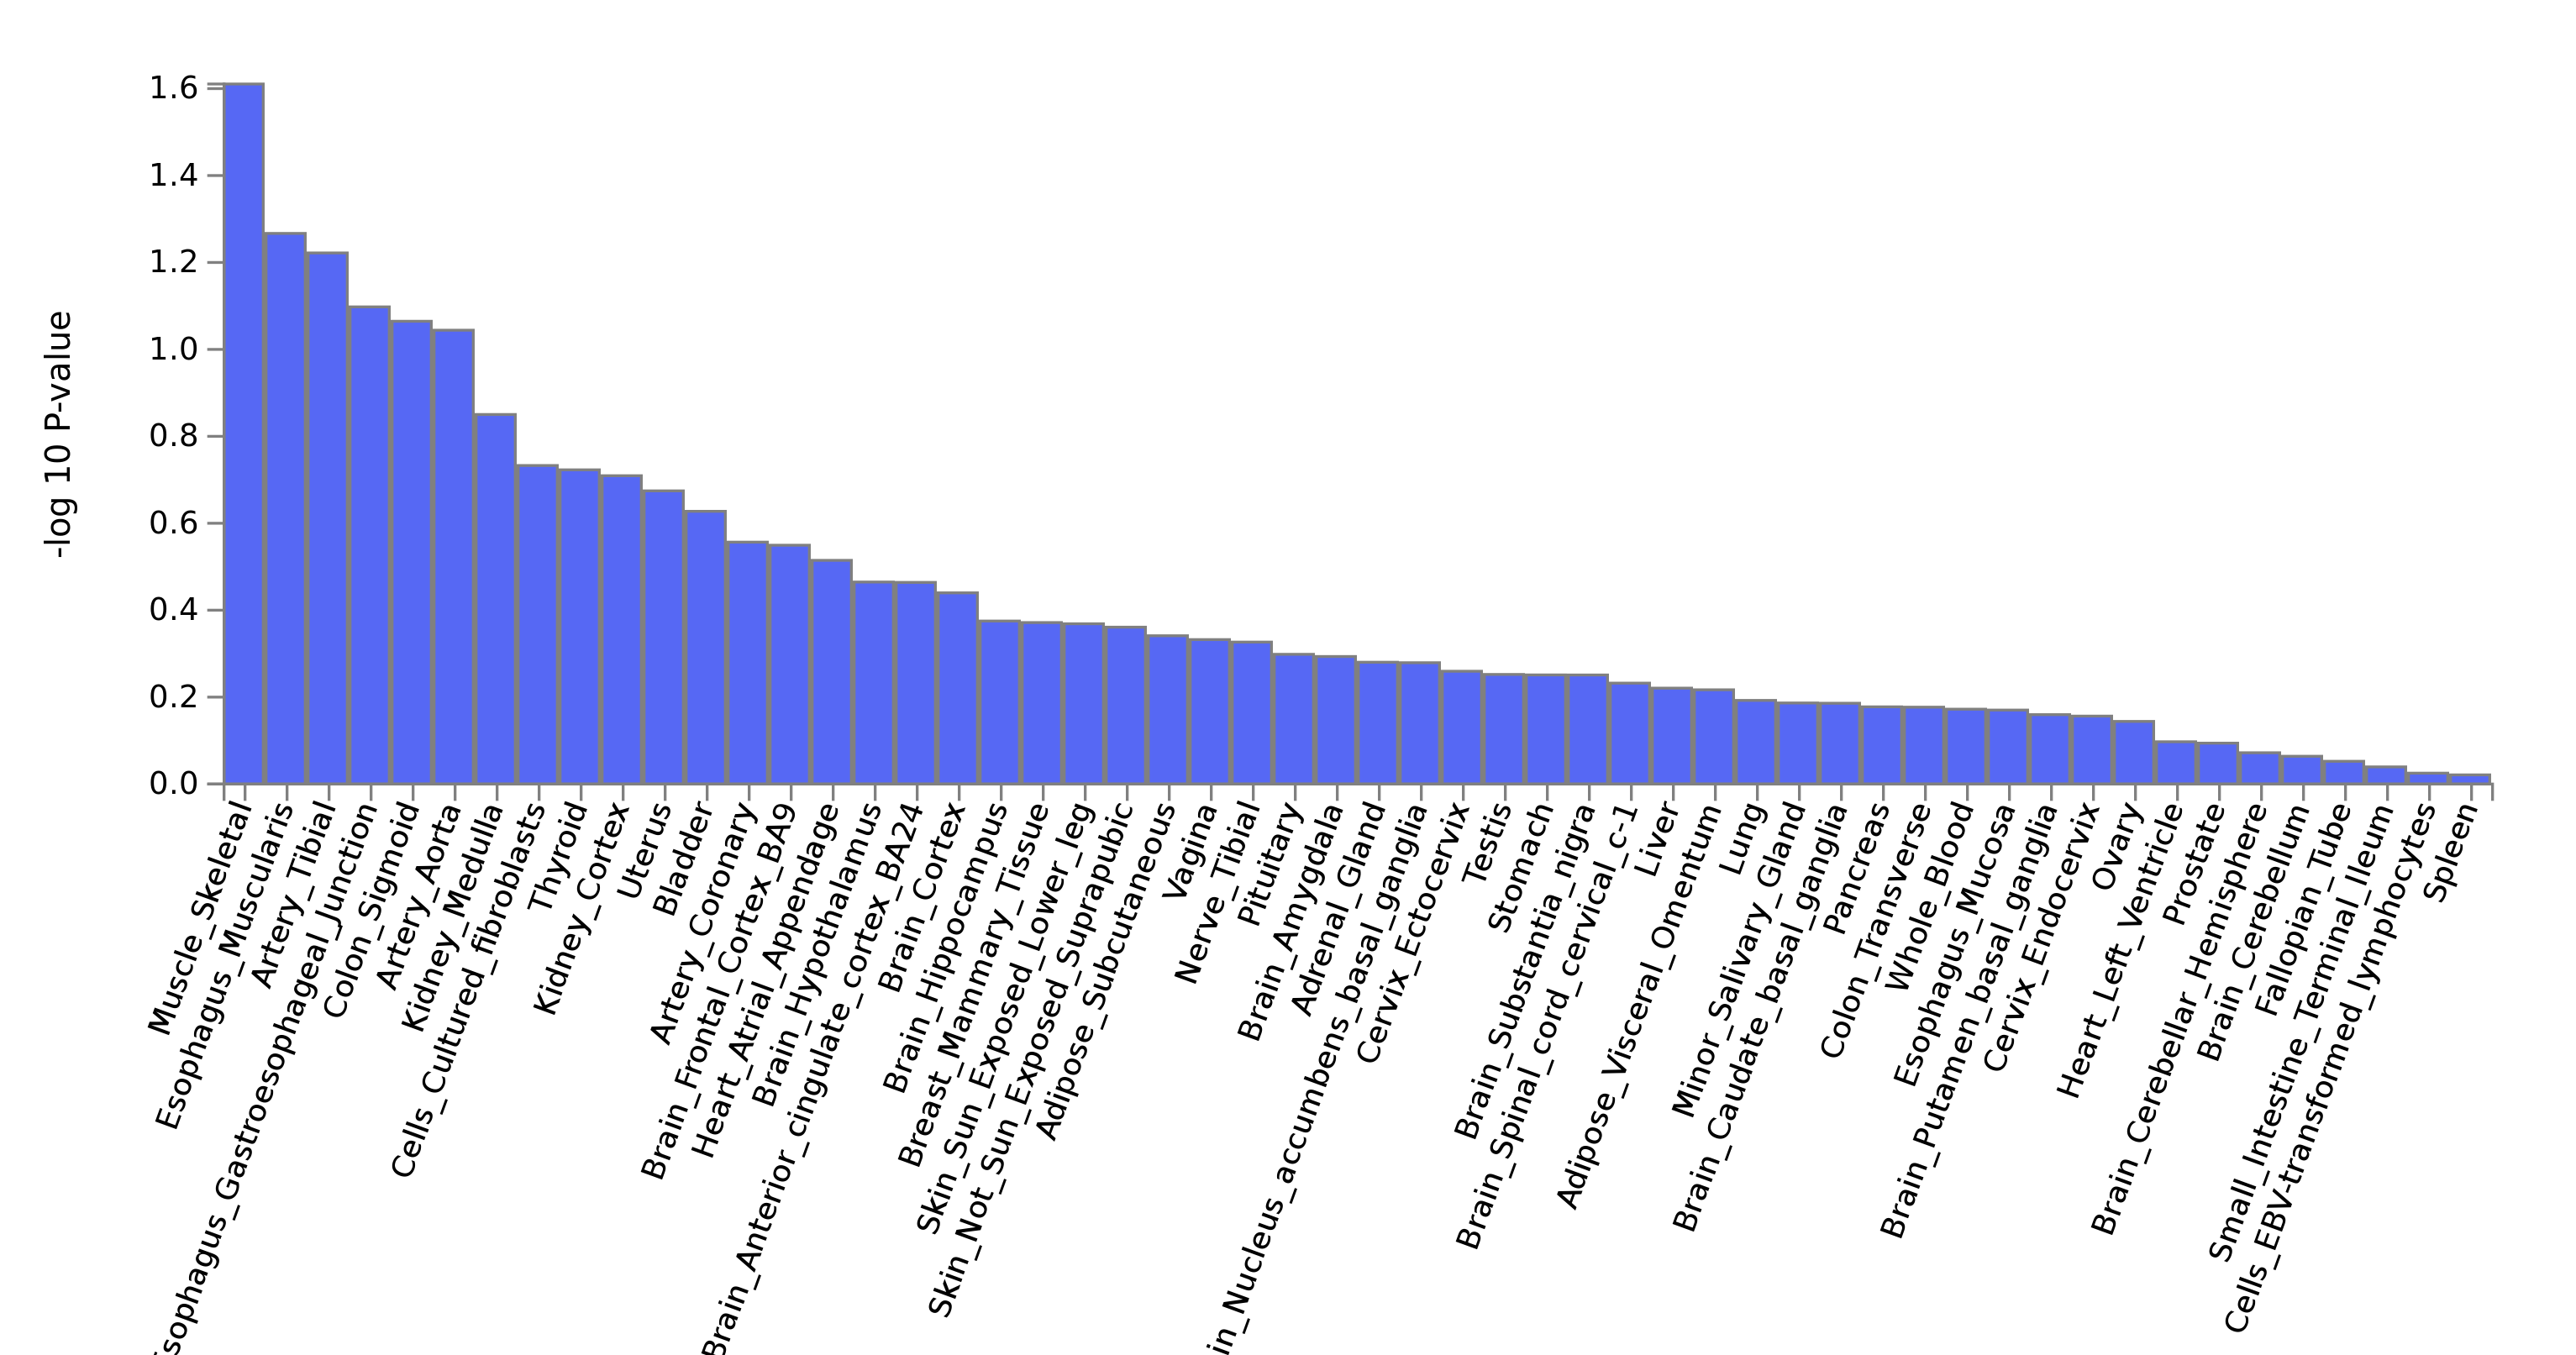
\includegraphics[width=0.85\textwidth]{images/SFig4.png}
  \caption{Gene-property analysis for issue specificity PGS-Only variants}
\end{figure}

\begin{figure}[h!]
  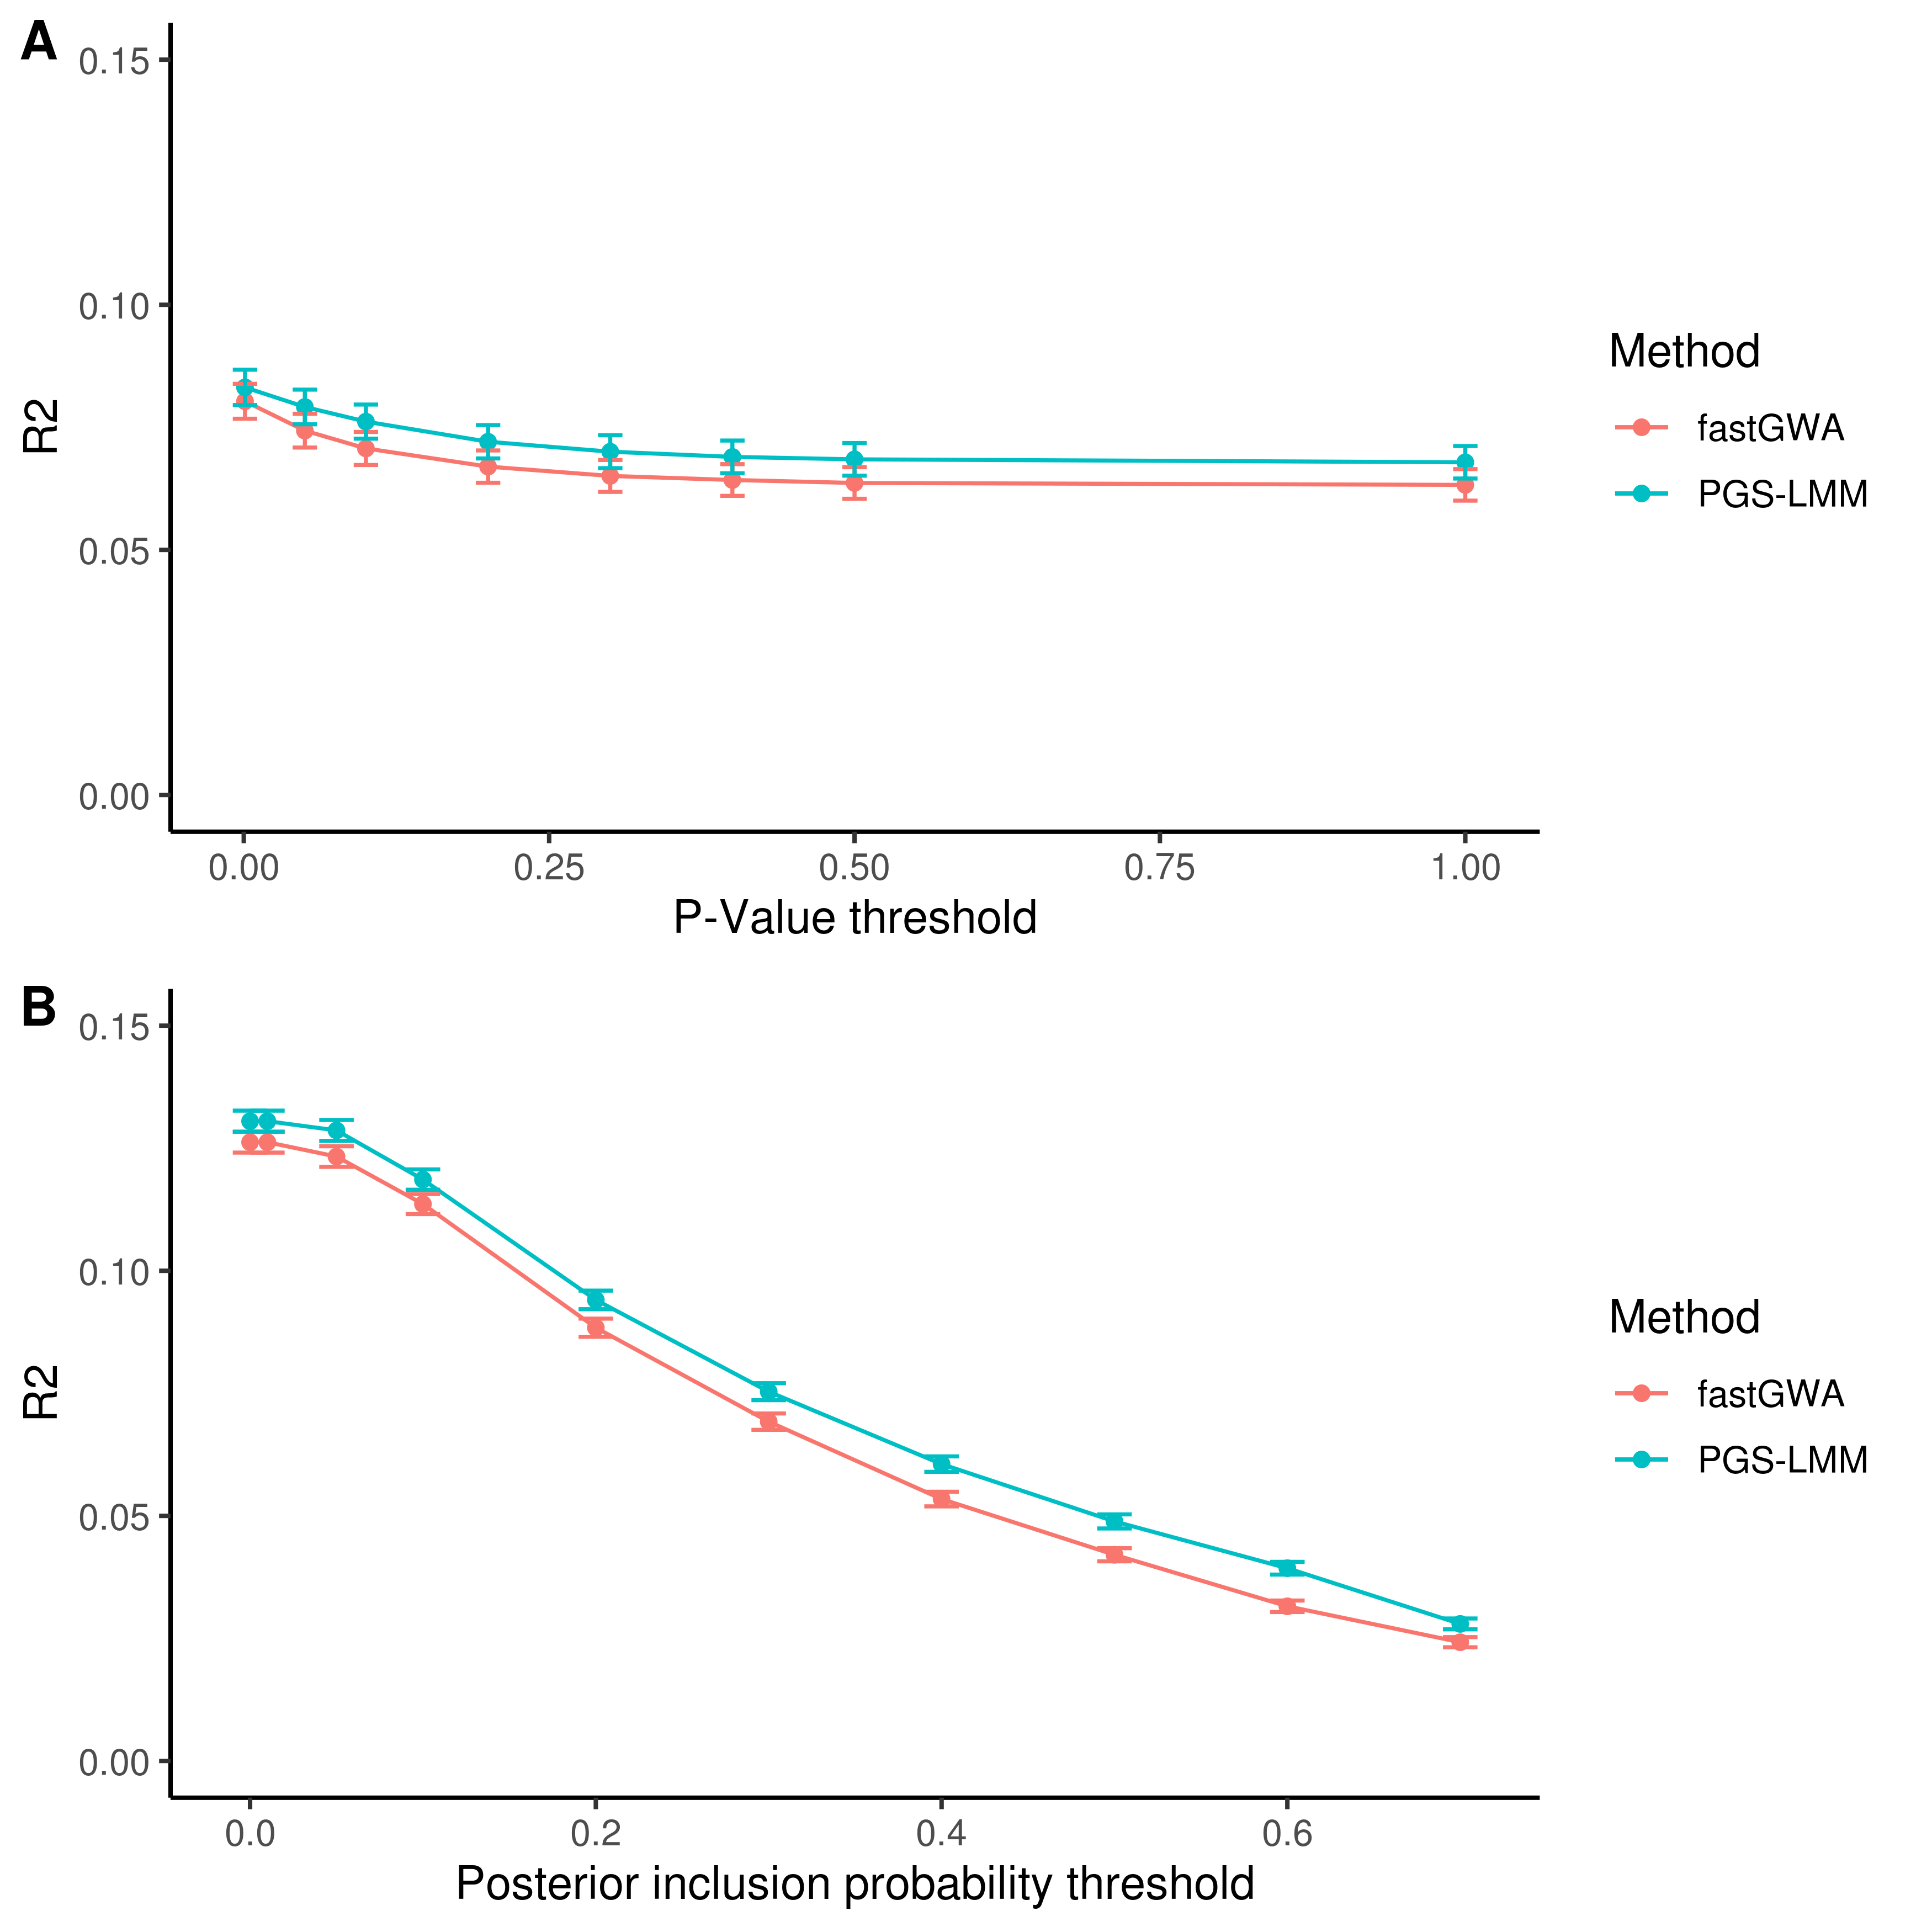
\includegraphics[width=0.85\textwidth]{images/SFig5.png}
  \caption{P+T prediction (A) across range of p value thresholds for each method Bayesian inference prediction (B) across PIP scores. Summary statistics are calculated on the 20\% training data}
\end{figure}

\begin{figure}[h!]
  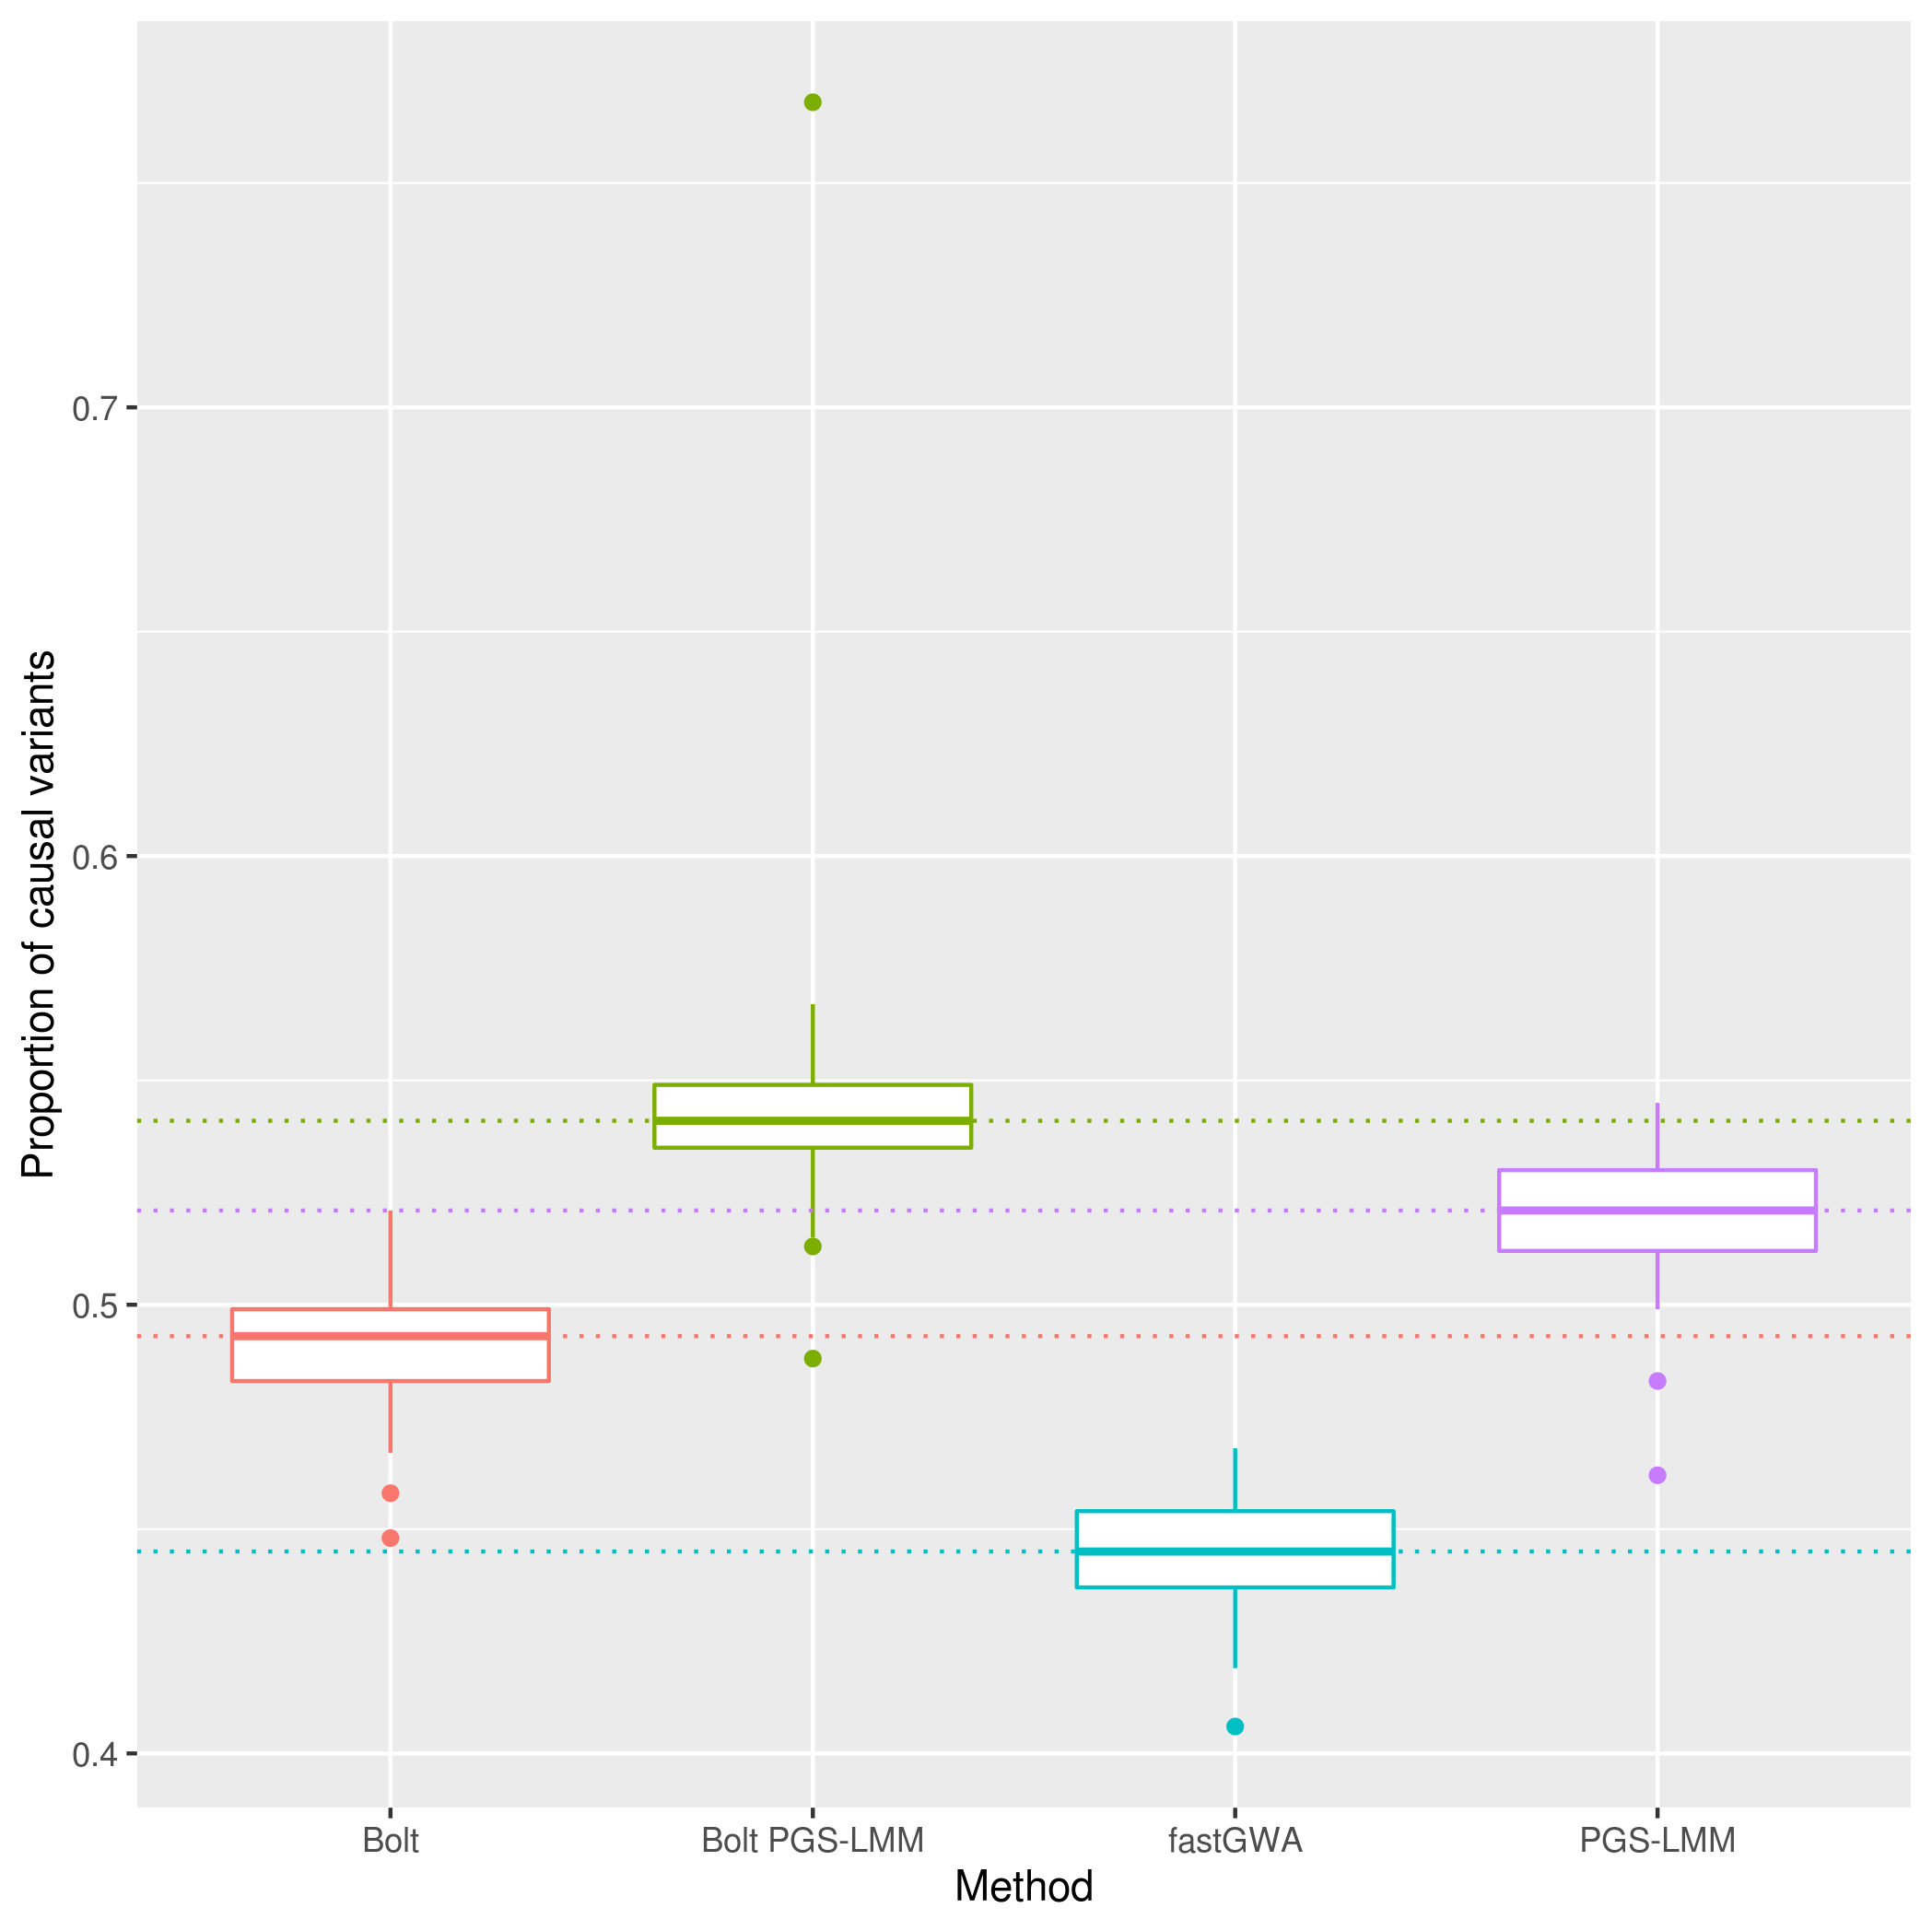
\includegraphics[width=0.85\textwidth]{images/SFig6.png}
  \caption{Proportion of causal variants identified by BOLT-LMM, BOLT-LMM PGS-LMM, fastGWA and fastGWA PGS-LMM across 100 simulations}
\end{figure}




\begin{table}[h!]
\renewcommand{\thetable}{S\arabic{table}}
\centering
\caption{Fishers exact test for expected number of variants in each minor allele frequency bin}
\resizebox{1.2\textwidth}{!}{\hskip-4.0cm\begin{tabular}{rlrrrrrrrlr} 
  \hline
 & Bin & Prop. fastGWA & Tot. fastGWA & Total fastGWA bin & Prop. PGS-LMM & Tot. PGS-LMM & Tot. PGS-LMM bin & OR & CI & P.value \\ 
  \hline
1 & $<$1\% & 0.01 & 126210 & 1096 & 0.02 & 30682 & 650 & 2.44 & 2.209-2.693 & 0.00 \\ 
  2 & 1-5\% & 0.10 & 115763 & 11543 & 0.10 & 28598 & 2734 & 0.96 & 0.9175-1.002 & 0.06 \\ 
  3 & 5-10\% & 0.14 & 111480 & 15826 & 0.15 & 27312 & 4020 & 1.04 & 0.9988-1.076 & 0.06 \\ 
  4 & 10-20\% & 0.28 & 99667 & 27639 & 0.36 & 22969 & 8363 & 1.31 & 1.276-1.351 & 0.00 \\ 
  5 & 20-50\% & 1.27 & 56104 & 71202 & 0.99 & 15767 & 15565 & 0.78 & 0.7588-0.7974 & 0.00 \\ 
   \hline
\end{tabular}}
\end{table}

\begin{table}[h!]
\vspace{-7.5em}%
\renewcommand{\thetable}{S\arabic{table}}
\centering
\caption{Gene-property analysis results}
\begin{tabular}{rlrrrrr}
  \hline
 & Tissue & N Genes & Beta & Beta Std. & Se & P \\ 
  \hline
1 & Muscle Skeletal & 2049 & 0.02 & 0.04 & 0.01 & 0.02 \\ 
  2 & Esophagus Muscularis & 2049 & 0.03 & 0.05 & 0.02 & 0.05 \\ 
  3 & Artery Tibial  & 2049 & 0.02 & 0.04 & 0.01 & 0.06 \\ 
  4 & Esophagus Gastroesophageal J.. & 2049 & 0.03 & 0.05 & 0.02 & 0.08 \\ 
  5 & Colon Sigmoid & 2049 & 0.03 & 0.05 & 0.02 & 0.09 \\ 
  6 & Artery Aorta  & 2049 & 0.02 & 0.04 & 0.01 & 0.09 \\ 
  7 & Kidney Medulla & 2049 & 0.02 & 0.03 & 0.02 & 0.14 \\ 
  8 & Cells Cultured fibroblasts & 2049 & 0.01 & 0.02 & 0.01 & 0.18 \\ 
  9 & Thyroid & 2049 & 0.01 & 0.02 & 0.02 & 0.19 \\ 
  10 & Kidney Cortex & 2049 & 0.01 & 0.02 & 0.02 & 0.20 \\ 
  11 & Uterus & 2049 & 0.01 & 0.03 & 0.02 & 0.21 \\ 
  12 & Bladder  & 2049 & 0.02 & 0.03 & 0.02 & 0.24 \\ 
  13 & Artery Coronary & 2049 & 0.01 & 0.02 & 0.02 & 0.28 \\ 
  14 & Brain Frontal Cortex BA9 & 2049 & 0.01 & 0.01 & 0.01 & 0.28 \\ 
  15 & Heart Atrial Appendage & 2049 & 0.01 & 0.01 & 0.02 & 0.31 \\ 
  16 & Brain Hypothalamus & 2049 & 0.01 & 0.01 & 0.01 & 0.34 \\ 
  17 & Brain Anterior cing. & 2049 & 0.00 & 0.01 & 0.01 & 0.34 \\ 
  18 & Brain Cortex & 2049 & 0.00 & 0.01 & 0.01 & 0.36 \\ 
  19 & Brain Hippocampus & 2049 & 0.00 & 0.00 & 0.01 & 0.42 \\ 
  20 & Breast Mammary Tissue & 2049 & 0.00 & 0.01 & 0.02 & 0.43 \\ 
  21 & Skin Sun Exposed Lower leg & 2049 & 0.00 & 0.00 & 0.01 & 0.43 \\ 
  22 & Skin Not Sun Exposed Suprapu... & 2049 & 0.00 & 0.00 & 0.01 & 0.44 \\ 
  23 & Adipose Subcutaneous & 2049 & 0.00 & 0.00 & 0.02 & 0.46 \\ 
  24 & Vagina  & 2049 & 0.00 & 0.00 & 0.02 & 0.47 \\ 
  25 & Nerve Tibial  & 2049 & 0.00 & 0.00 & 0.02 & 0.47 \\ 
  26 & Pituitary  & 2049 & -0.00 & -0.00 & 0.01 & 0.50 \\ 
  27 & Brain Amygdala & 2049 & -0.00 & -0.00 & 0.01 & 0.51 \\ 
  28 & Adrenal Gland & 2049 & -0.00 & -0.00 & 0.02 & 0.52 \\ 
  29 & Brain Nucleus accumbens basa... & 2049 & -0.00 & -0.00 & 0.01 & 0.53 \\ 
  30 & Cervix Ectocervix & 2049 & -0.00 & -0.00 & 0.02 & 0.55 \\ 
  31 & Testis  & 2049 & -0.00 & -0.00 & 0.01 & 0.56 \\ 
  32 & Stomach  & 2049 & -0.00 & -0.01 & 0.02 & 0.56 \\ 
  33 & Brain Substantia nigra & 2049 & -0.00 & -0.00 & 0.01 & 0.56 \\ 
  34 & Brain Spinal cord cervical c... & 2049 & -0.00 & -0.00 & 0.01 & 0.59 \\ 
  35 & Liver & 2049 & -0.00 & -0.00 & 0.01 & 0.60 \\ 
  36 & Adipose Visceral Omentum & 2049 & -0.00 & -0.01 & 0.02 & 0.61 \\ 
  37 & Lung & 2049 & -0.01 & -0.01 & 0.02 & 0.64 \\ 
  38 & Minor Salivary Gland & 2049 & -0.01 & -0.01 & 0.02 & 0.65 \\ 
  39 & Brain Caudate basal ganglia & 2049 & -0.01 & -0.01 & 0.01 & 0.65 \\ 
  40 & Pancreas & 2049 & -0.01 & -0.01 & 0.01 & 0.66 \\ 
  41 & Colon Transverse & 2049 & -0.01 & -0.01 & 0.02 & 0.67 \\ 
  42 & Whole Blood & 2049 & -0.00 & -0.01 & 0.01 & 0.67 \\ 
  43 & Esophagus Mucosa & 2049 & -0.01 & -0.01 & 0.01 & 0.68 \\ 
  44 & Brain Putamen basal ganglia & 2049 & -0.01 & -0.01 & 0.01 & 0.69 \\ 
  45 & Cervix Endocervix & 2049 & -0.01 & -0.02 & 0.02 & 0.70 \\ 
  46 & Ovary & 2049 & -0.01 & -0.02 & 0.02 & 0.72 \\ 
  47 & Heart Left Ventricle & 2049 & -0.01 & -0.02 & 0.02 & 0.80 \\ 
  48 & Prostate & 2049 & -0.02 & -0.03 & 0.02 & 0.81 \\ 
  49 & Brain Cerebellar Hemisphere & 2049 & -0.01 & -0.02 & 0.01 & 0.85 \\ 
  50 & Brain Cerebellum & 2049 & -0.01 & -0.02 & 0.01 & 0.86 \\ 
  51 & Fallopian Tube & 2049 & -0.02 & -0.04 & 0.02 & 0.89 \\ 
  52 & Small Intestine Terminal Ile... & 2049 & -0.02 & -0.04 & 0.02 & 0.91 \\ 
  53 & Cells EBV-transformed lympho... & 2049 & -0.01 & -0.02 & 0.01 & 0.94 \\ 
  54 & Spleen & 2049 & -0.02 & -0.04 & 0.01 & 0.95 \\ 
   \hline
 \vspace{-151pt}
\end{tabular}
\end{table}

\begin{table}[h!]
\renewcommand{\thetable}{S\arabic{table}}
\centering
\caption{Prediciton results for 74,000 top independent loci in each method}
\resizebox{\textwidth}{!}{\begin{tabular}{rlrrrrrr}
  \hline
 & Set & Threshold & $R^2$ & P & Coefficient & Standard.Error & Num SNP \\
  \hline
1 & fastGWA & 0.00 & 0.13 &   0 & 8956.95 & 80.34 & 15750 \\
  2 & fastGWA & 0.05 & 0.13 &   0 & 29309.80 & 259.44 & 72216 \\
  3 & fastGWA & 0.10 & 0.13 &   0 & 29886.20 & 264.36 & 74000 \\
  4 & PGS-LMM & 0.00 & 0.13 &   0 & 11044.80 & 97.52 & 17856 \\
  5 & PGS-LMM & 0.05 & 0.14 &   0 & 35111.00 & 298.84 & 74000 \\
   \hline
\end{tabular}}
\end{table}

\end{document}
